\chapter{Stanovení požadavků návrhu zařízení}


Účelem tohoto projektu je rozšířit přístupový systém firmy IMA o IoT, aby bylo možné snímat veličiny jako je teplota, vlhkost, atd. bezdrátovými senzory rozmístěnými po budově.
Práce tedy zahrnuje návrh, realizace a otestování gatewaye, která shromažďuje data z bezdrátových koncových zařízení a přeposílá je na control panel přístupového systému. 
Předpokládá se, že koncová zařízení jsou senzory nebo aktuátory napájeny z baterie, tudíž pro jejich dlouhodobou životnost je kladen důraz na nízkou spotřebu vybrané bezdrátové technologie.

% \begin{figure}[!h]
%     \centering
%     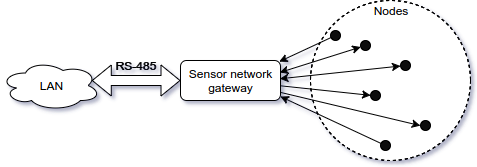
\includegraphics[width=1\textwidth]{01}
%     \caption{Blokový diagram funkce gatewaye}
%     \label{fig:block diagram of the system}
% \end{figure}


\section{Přístupové systémy}
Přístupové systémy jsou elektronické systémy řídící skrze síť přístup uživatelů do budov či objektů na základě ověření jejich identity \cite{accessControlSystem_eiprocus}.
V obrázku \ref{fig:Access control system architecture} je znázorněn příklad infrastruktury přístupového systému.

\begin{figure}[!h]
    \centering
    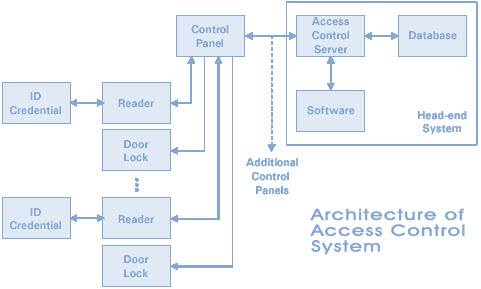
\includegraphics[width=1\textwidth]{Architetcture-of-Access-Control-System}
    \caption{Příklad architektury přístupového systému \cite{accessControlSystem_eiprocus}}
    \label{fig:Access control system architecture}
\end{figure}

"ID Credential" je identifikátor uživatele, např. RFID tag, otisk prstu, QR kód atd.
Reader slouží k sejmutí dat identifikátoru uživatele a odeslání do "control panelu"
Door lock slouží k ovládání přístupu uživatele do objektu.
Control panel vytváří rozhranní mezi "Access control system" a dvojcemi readerů a door locků. 
Obvykle vytváří síť například RS485, kde jsou zapojeny jednotky až desítky těchto dvojíc. 
V jednom systému může být jeden nebo více control panelů vytvářejících síť o jedné nebo více dvojicích reader a door lock.
Control panel komunikuje s access control systémem například přes ethernet na bázi protokolu TCP/IP.
Databáze obsahuje uživatelská ID.
Na access control serveru je spuštěn software umožňující spravování databáze a komunikaci se všemi control panely systému.
Prokáže-li se uživatel pomocí ID credential readeru, reader sejme ID uživatele a odešle na control panel, který jej následně přepošle na access control server.
Software access control vyhledá přijaté user ID v databázi a je-li nalezeno, pošle na odpovídající control panel příkaz k sepnutí odpovídajícího door locku.




\section{Implementace IoT do přístupového systému firmy IMA}
\label{sec:Implementace IoT do přístupového systému firmy IMA}
V infrastruktuře přístupového systému v obr. \ref{fig:Access control system architecture} je reader nahrazen gatewayí a ID credential bezdrátovým senzorem. 
Gateway pak komunikuje s control panelem přes rozhranní RS485 s proprietárním síťovým protokolem navrženým ve firmě IMA. 
Stávajcí přístupový systém je navržen tak, že po spuštění připojeného readeru je mu ze serveru předán seznám offline RFID karet. 
Pro gateway to je seznam adres koncových zařízení senzorové sítě. 
V případě, že uživatel přiloží ID credential odpovídající některému ze seznamu offline karet, reader přepošle příkaz "průchod".
Ekvivalentně to platí pro gateway. 
V případě že gateway přijme packet od koncového zařízení s daty ze senzorů a adresa koncového zařízení je obsažena v seznamu adres koncových zařízení,
gateway odešle příkaz "průchod" obsahující adresu koncového zařízení a data koncového zařízení.
Problém je ale v tom, že příkaz "průchod" má kapacitu na data koncového zařízení pouze 6 bytů.
Rošiřování vlastností tohoto protokolu by znamenalo mnoho komplikací, 
cílem je tedy implementace gatewaye tak, aniž by bylo nutné protokol rozšiřovat.


% - popiste infrastrukturu pristupovych systemu (obrazek a popis jednotlivych bloku), a jednak jejich vyuziti, zda se pouzivaji i na neco jineho - opet clanky, ten obr. 3.1 neni dostatecny pro clanek. Mam na mysli toto:
% https://www.elprocus.com/understanding-about-types-of-access-control-systems/
% https://en.wikipedia.org/wiki/Access_control#Access_control_system_topologies